\documentclass[../../main.tex]{subfiles}
\begin{document}

\begin{flushright}
  \footnotesize\textit{【自動文字起こし・要確認】}
\end{flushright}

% Source: handwritten.pdf 第1問．
{\bf [解]}
点Aを始点とする位置ベクトルを小文字で表す．仮定より
\begin{align}
  \boldsymbol{c}\cdot(\boldsymbol{c}-\boldsymbol{b})&=0,\\
  \boldsymbol{d}\cdot(\boldsymbol{d}-\boldsymbol{b})&=0,\\
  \boldsymbol{b}\cdot(\boldsymbol{d}-\boldsymbol{c})&=0.
\end{align}
$\boldsymbol{m}=\dfrac{\boldsymbol{c}+\boldsymbol{d}}{2}$だから
\begin{align}
  \overrightarrow{AM}\cdot\overrightarrow{CD}
  &=\dfrac{1}{2}(\boldsymbol{c}+\boldsymbol{d})\cdot(\boldsymbol{d}-\boldsymbol{c})\\
  &=\dfrac{1}{2}(|\boldsymbol{d}|^2-|\boldsymbol{c}|^2)\\
  &=\dfrac{1}{2}(\boldsymbol{b}\cdot\boldsymbol{d}-\boldsymbol{b}\cdot\boldsymbol{c})=0.
\end{align}
よって$AM\perp CD$である．$AB\perp CD$でもあるから，平面ABMは直線CDと垂直である．
\begin{figure}[H]
  \begin{center}
    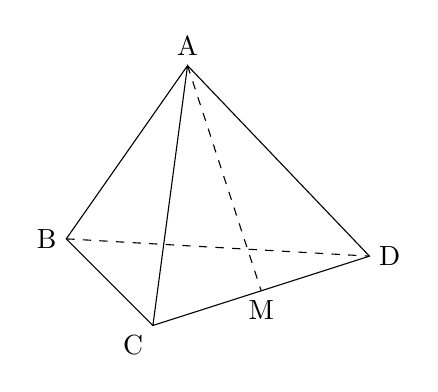
\begin{tikzpicture}[scale=1.1]
      \coordinate (A) at (1.4,3);\coordinate (B) at (0,1);\coordinate (C) at (1,0);\coordinate (D) at (3.5,.8);\coordinate (M) at (2.25,.4);
      \draw (A)--(B)--(C)--(D)--(A)--(C);\draw[dashed] (B)--(D) (A)--(M);
      \node[above] at (A){A};\node[left] at (B){B};\node[below left] at (C){C};\node[right] at (D){D};\node[below] at (M){M};
    \end{tikzpicture}
  \end{center}
  \caption{四面体ABCDと辺CDの中点M}
\end{figure}

\end{document}
